\documentclass[10pt]{article}

\input{/Users/gabesekeres/Dropbox/LaTeX_Docs/pset_preamble.tex}

\course{ECON 6140}
\pset{3}
\begin{document}
\maketitle

\section*{Health inequality and mitigation tools}


\begin{enumerate}
	\item If we impose risk-sharing, which follows directly from the social planner caring for each type equally, the utilitarian social planner solves the problem \[\max_{\{c_t,h_t,x_t,k_{t+1},\pi_t\}} \sum_{t=0}^\infty \frac{1}{2}\parl (\beta \pi_t)^t + \beta^t\parr u(c_t)\]subject to \begin{align*} k_{t+1} &= x_t + (1-\delta)k_t \\ y_t &= Ak_t^\alpha \\ y_t &= c_t + h_t + x_t \\ \pi_t &= f\parl \frac{h_t}{y_t}\parr \\ c_t,h_t,x_t,k_{t+1} &\ge 0 \\ k_0 &> 0 \text{ given} \end{align*}Their Lagrangian is \begin{align*}\mathcal{L} = \sum_{t=0}^\infty \beta^t \Bigg\{ &(\pi_t^t + 1)u(c_t) + \lambda_t \parl x_t + (1-\delta)k_t - k_{t+1} \parr \\ &+ \theta_t \parl A k_t^\alpha - c_t - h_t - x_t\parr + \mu_t\parl f\parl \frac{h_t}{Ak_t^\alpha}\parr - \pi_t\parr \Bigg\}\end{align*}which admits first order conditions\begin{align*} 0 &= (\pi^t_t + 1)u'(c_t) - \theta_t &&(c_t) \\ 0 &= -\theta_t + \frac{\mu_t}{Ak_t^\alpha} f'\parl \frac{h_t}{Ak_t^\alpha}\parr &&(h_t) \\ 0 &= \lambda_t - \theta_t &&(x_t) \\ 0 &= -\lambda_t + \beta \barl \lambda_{t+1}(1-\delta) + \theta_{t+1}\alpha Ak_{t+1}^{\alpha-1} - \frac{\mu_{t+1} \alpha h_{t+1}}{Ak_{t+1}^{\alpha + 1}} f'\parl \frac{h_{t+1}}{Ak_{t+1}^\alpha}\parr\barr &&(k_{t+1}) \\ 0 &= t\pi^{t-1}_t u(c_t) - \mu_t &&(\pi_t) \end{align*}Substituting for the Lagrange multipliers in the fourth first order condition, we get \[(\pi_t^t + 1)u'(c_t) = \beta (\pi_{t+1}^t + 1)u'(c_{t+1})\barl (1-\delta) + \alpha Ak_{t+1}^{\alpha - 1} - \frac{\alpha h_{t+1}}{k_{t+1}}\barr\]In steady state, this becomes\[1 = \beta \barl (1-\delta) + \alpha A (k\opt)^{\alpha-1} - \alpha h\opt (k\opt)^{-1}\barr\]and feasibility requires \[c\opt + h\opt + \delta k\opt = A(k\opt)^\alpha \]We have two equations for three unknowns ($h\opt$, $k\opt$, and $c\opt$). To get a third equation, we use the first order condition with respect to $h$ and the definition of $\pi$, which, in steady state, is\[\theta = \frac{\mu}{A (k\opt)^\alpha} f'\parl \frac{h\opt}{A (k\opt)^\alpha}\parr \Longrightarrow (f(\cdot)^t + 1)u'(c\opt) = \frac{tf(\cdot)^{t-1}u(c\opt)}{A (k\opt)^\alpha}f'(\cdot)\]which, substituting from the feasibility constraint, becomes\[\barl f\parl \frac{h\opt}{A (k\opt)^\alpha}\parr^t + 1\barr u'(A(k\opt)^\alpha - \delta k\opt - h\opt) = \frac{tf\parl \frac{h\opt}{A (k\opt)^\alpha}\parr^{t-1}u(A(k\opt)^\alpha - \delta k\opt - h\opt)}{A (k\opt)^\alpha}f'\parl \frac{h\opt}{A (k\opt)^\alpha}\parr\]With the Euler equation\[1 = \beta \barl (1-\delta) + \alpha A (k\opt)^{\alpha-1} - \alpha h\opt (k\opt)^{-1}\barr\]this is a characterization of $k\opt$ and $h\opt$. However, it cannot be further reduced to remove the $t$ term. Instead, we will impose a steady state, making the assumption that a nontrivial steady state exists in which $\pi_t = \pi \in (0,1)$ for all $t$. In this case, the planner's objective function becomes, using the properties of geometric series, \[\max_{\{c,h,x,k,\pi\}} \frac{1}{2} \sum_{t=0}^\infty (\beta\pi)^t u(c) + \frac{1}{2} \sum_{t=0}^\infty \beta^t u(c) \equiv \max_{\{c,h,x,k,\pi\}} \frac{1}{2} \parl \frac{1}{1-\beta\pi} + \frac{1}{1-\beta}\parr u(c)\]subject to \begin{align*} k &= x + (1-\delta)k \\ y &= Ak^\alpha \\ y &= c + h + x \\ \pi &= f(h / y) \\ c,h,x,k &\ge 0 \end{align*}So the Lagrangian is\[ \mathcal{L} = \frac{1}{2} \parl \frac{1}{1-\beta\pi} + \frac{1}{1-\beta}\parr u(c) + \lambda (x - \delta k) + \theta(Ak^\alpha - c - h - x) + \mu \parl f(h / Ak^\alpha) - \pi\parr \]which admits first order conditions \begin{align*} 0 &= \frac{1}{2} \parl \frac{1}{1-\beta\pi} + \frac{1}{1-\beta}\parr u'(c) - \theta &&(c) \\0 &= -\theta + \frac{\mu}{Ak^\alpha} f'(h / Ak^\alpha) &&(h) \\ 0 &= \lambda - \theta &&(x) \\ 0 &= -\delta \lambda + \theta \alpha Ak^{\alpha-1} - \mu\frac{h}{Ak^{\alpha+1}}f'(h/Ak^\alpha) &&(k) \\0 &= \frac{\beta}{2} \frac{1}{(1-\beta\pi)^2}u(c) - \mu &&(\pi) \end{align*}Substituting the Lagrange multipliers in the fourth condition, it becomes \[\delta  = \alpha Ak^{\alpha-1} -\frac{h}{k} \Longrightarrow h = \alpha Ak^\alpha - \delta k\]So from feasibility, we have \[c = Ak^\alpha - (\alpha Ak^\alpha - \delta k) - \delta k = (1-\alpha)Ak^\alpha \]Meaning that consumption is a constant fraction of output. Finally, combining a few conditions, we get that \[ \frac{\beta}{(1-\beta\pi)^2}u((1-\alpha)Ak^\alpha) = \parl \frac{1}{1-\beta\pi} + \frac{1}{1-\beta}\parr \frac{Ak^\alpha}{f'(\alpha - \delta k / Ak^\alpha)}u'((1-\alpha)Ak^\alpha)\]Which precisely characterizes $k$ in terms of the model primitives once we have functional forms for $u$ and $f$.
	\item The immortal households' problem reduces to the traditional \[\max_{\{c_t,x_t,k_{t+1}\}} \sum_{t=0}^\infty \beta^t u(c_t) \]subject to \begin{align*} k_{t+1} &= x_t + (1-\delta)k_t \\ y_t &= Ak_t^\alpha \\ y_t &= c_t + x_t \\ c_t,x_t,k_{t+1} &\ge 0\end{align*}where we trivially impose that $h_t = 0$ for all $t$. The Lagrangian is \[\mathcal{L} = \sum_{t=0}^\infty \beta^t \Bigg\{u(c_t) + \lambda_t \parl x_t + (1-\delta)k_t - k_{t+1}\parr + \theta_t \parl Ak_t^\alpha - c_t - x_t\parr \Bigg\}\]which admits the first order conditions \begin{align*} 0 &= u'(c_t) - \theta_t &&(c_t) \\ 0 &= \lambda_t - \theta_t &&(x_t) \\ 0 &= -\lambda_t + \beta \barl \lambda_{t+1}(1-\delta) + \theta_{t+1} \alpha Ak_{t+1}^{\alpha-1}\barr &&(k_{t+1})\end{align*}so the Euler equation is \[u'(c_t) = \beta u'(c_{t+1})\barl (1-\delta) + \alpha Ak_{t+1}^{\alpha-1}\barr\]which in steady state becomes\[1 = \beta\barl (1-\delta) + \alpha Ak^{\alpha-1}\barr \Longrightarrow k = \parl\frac{\frac{1}{\beta} - (1-\delta)}{\alpha A}\parr^{\frac{1}{\alpha-1}}\]Meanwhile, the mortal households solve\[\max_{\{c_t,x_t,k_{t+1},h_t,\pi_t\}} \sum_{t=0}^\infty (\beta\pi_t)^t u(c_t) \]subject to\begin{align*} k_{t+1} &= x_t + (1-\delta)k_t \\ y_t &= Ak_t^\alpha \\ y_t &= c_t + h_t + x_t \\ \pi_t &= f(h_t / y_t) \\ c_t,h_t,x_t,k_{t+1} &\ge 0\end{align*}As in part (1), the first order conditions will require taking the derivative with respect to $\pi_t$, so in order to find a steady state we again assume that one exists, in which $\pi_t = \pi \in (0,1)$ for all $t$. The problem becomes \[\max_{\{c,h,x,k,\pi\}} \frac{1}{1-\beta\pi} u(c) \]subject to\begin{align*} k &= x + (1-\delta)k \\ y &= Ak^\alpha \\ y &= c + h + x \\ \pi &= f(h/y) \\ c,h,x,k &\ge 0 \end{align*}So the Lagrangian is \[\mathcal{L} = \frac{1}{1-\beta\pi} u(c) + \lambda(x - \delta k) + \theta (Ak^\alpha - c - h - x) + \mu(f(h / Ak^\alpha)-\pi)\]which admits first order conditions\begin{align*} 0 &= \frac{u'(c)}{1-\beta\pi} - \theta &&(c) \\ 0 &= -\theta + \frac{\mu}{Ak^\alpha} f'(h/Ak^\alpha) &&(h) \\ 0 &= \lambda - \theta &&(x) \\ 0 &= \lambda \delta + \theta \alpha Ak^{\alpha-1} + \mu \frac{h}{Ak^{\alpha+1}} f'(h/Ak^{\alpha}) &&(k) \\0 &= \frac{\beta}{(1-\beta\pi)^2} u(c) - \mu &&(\pi)\end{align*}As in the social planner's problem, we have that \[\delta = \alpha Ak^{\alpha-1} - \frac{h}{k} \Longrightarrow h = \alpha Ak^\alpha - \delta k \]and from feasibility, we have that\[c = Ak^\alpha - (\alpha Ak^\alpha - \delta k ) - \delta k = (1-\alpha )Ak^\alpha\]So as above, consumption is a constant fraction of output. Finally, combining conditions, we have that $k$ is precisely characterized by \[\frac{\beta}{1-\beta\pi} u(c) = u'(c) \frac{Ak^\alpha}{f'(h/Ak^\alpha)}\]
	\item In the social planner's problem, the health investment to output ratio is \[\frac{h}{y} = \frac{\alpha Ak^\alpha - \delta k}{Ak^\alpha} = \alpha - \frac{\delta k }{Ak^\alpha}\]Meanwhile in the competitive equilibrium, the immortal households invest 0 and the mortal households invest $\alpha Ak^\alpha - \delta k$. Assuming that the fraction of mortal households is $\gamma \in (0,1)$, we have that the health investment to output ratio at some total capital level $k$ is \[\frac{(1-\gamma) \cdot 0 + \gamma \cdot h}{y} = \gamma \alpha - \frac{\gamma \delta k}{Ak^\alpha}\]which is a fixed proportion $\gamma$ of the health investment in the social planner's problem. Intuitively, this is because the immortal households do not care about the investment in health at all.
	\item If the government bans pesticides, all households will be immortal. The planner's problem becomes (assuming risk-sharing, as before) \[\max_{\{c_t,x_t,k_{t+1}\}} \sum_{t=0}^\infty \beta^t u(c_t)\]subject to \begin{align*}k_{t+1} &= x_t + (1-\delta)k_t \\ y_t &= A'k_t^\alpha \\ y_t &= c_t + x_t \\ c_t,x_t,k_{t+1} &\ge 0\end{align*}Since there are no longer any returns to investing in health, we remove those conditions and set $h\opt = 0$ in steady state. Observe that this problem is identical to the problem the immortal households solve in the competitive equilibrium. The steady state investment in capital will be \[k\opt = \parl \frac{\frac{1}{\beta} - (1-\delta)}{\alpha A'}\parr^{\frac{1}{\alpha-1}}\]While we did not have a precise closed-form characterization above, we can say that this is strictly larger than the investment in part (1), since in part (1) the social planner invested positive amounts in health.
	\item From part (1), we have that in the steady state \[ \frac{\beta}{(1-\beta\pi)^2}u(c) = \parl \frac{1}{1-\beta\pi} + \frac{1}{1-\beta}\parr \frac{y}{f'(h/y)}u'(c)\]So we have that the value of life is \[\frac{u(c)}{u'(c)} = \frac{(1-\beta\pi)^2}{\beta} \parl \frac{1}{1-\beta\pi} + \frac{1}{1-\beta}\parr \frac{y}{f'(h/y)}\]Recall that the investment in health above is a direct function of $k$, which is defined implicitly by this expression. As the value of life increases, the optimal investment in capital will decrease and the optimal investment in health will increase, as we can see from the rightmost term. This makes implicit sense -- as life is more valuable, the social planner is willing to invest more to increase life.
\end{enumerate}






\section*{Saving policies: risk and non-homotheticities}

\begin{enumerate}
	\item The farmer's maximization problem can be written as \[\max_{\{c_t\}} \sum_{t=0}^\infty \beta^t \ln(c_t) \st \sum_{t=0}^\infty c_t= x_0\]Taking the value function as the attained maximum, we get that starting with endowment $x_t$ in period $t$, \[v(x_t) = \max_{c_t} \ln(c_t) + \beta v(x_t - c_t) \]so, rewriting in standard notation, we get that \[v(x) = \max_{c\in [0,x]} \ln(c) + \beta v(x - c)\]
	\item I discretized the initial endowment space with $1000$ points from $0$ to $100$, and calculated the value function for the farmer across that grid. The value function is plotted in Figure~\ref{fig:value_initial}. The code is included below this section. I added an absorbing state where $v(0)=0$. This will become relevant in part (3) of the problem, for now it causes some strangeness around low levels of the initial endowment but otherwise changes nothing. \begin{figure}[H] \centering 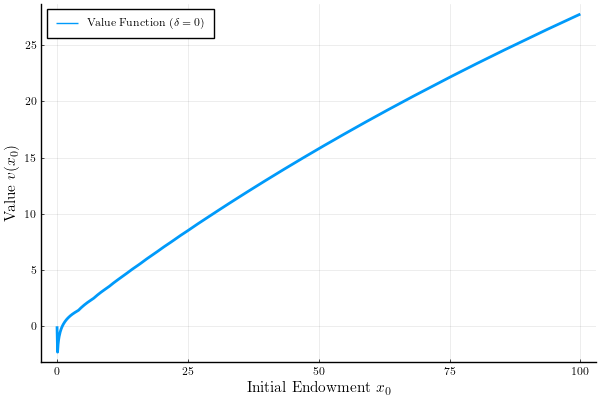
\includegraphics[width=10cm]{macro_hw3_code/value_function.png} \caption{Value to the Farmer (when $\delta = 0$)} \label{fig:value_initial}\end{figure}
	\item The farmer has a probability $\delta$ of losing the entire endowment each period. Of course, this runs into the immediate problem that $\log(0) = -\infty$, so any expected utility calculation would lead to, in expectation, $-\infty$ utility. Instead, we will manually set $v(0)=0$, and restrict the range of initial endowments to those where the value should be positive -- see above, where we set the minimum endowment at $2.5$. With this, the Bellman equation becomes \[v(x) = \max_{c \in [0,x]} \ln(c) + \beta \barl \delta v(0) + (1-\delta)v(x-c)\barr \]which simplifies to \[v(x) = \max_{c \in [0,x]} \ln(c) + \beta(1-\delta)v(x-c)\]We can rewrite the code to include this value function, and get Figure~\ref{fig:value_delta}. Note that the new value function is not a linear transformation of the old -- consumption patterns shift, putting more weight on the present, which reduces total value more than linearly. \begin{figure}[H] \centering 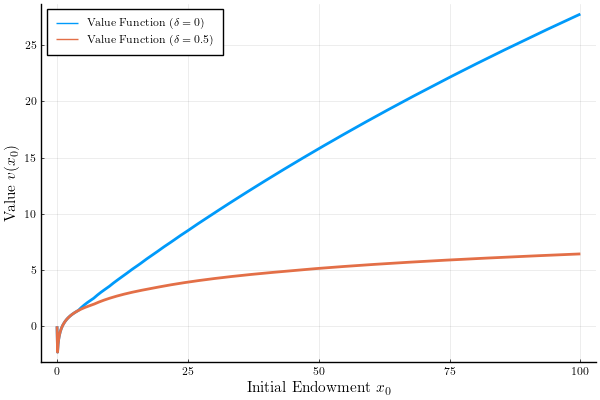
\includegraphics[width=10cm]{macro_hw3_code/value_function_delta.png} \caption{Value to the Farmer when $\delta = 0.5$} \label{fig:value_delta} \end{figure}
	\item If we now have a lower bound on the value function $\bar{c} = x_0 / 100$, we can represent the (non-homothetic) utility function as: \[u(c) = \begin{cases} \ln(c - \bar{c}) & c >\bar{c} \\ -\infty & c \le \bar{c}\end{cases}\]This admits the Bellman Equation \[v(x) = \max_{c \in [\bar{c},x]} \ln(c-\bar{c}) + \beta v(x - c)\]The value functions are plotted in Figure~\ref{fig:value_subs}. As we can see, there are no large differences at low initial endowment, but at higher levels of the initial endowment the farmer would clearly prefer to consume less than $\bar{c}$ in some periods, so we have further constrained their problem (which necessarily leads to less value). \begin{figure}[H] \centering 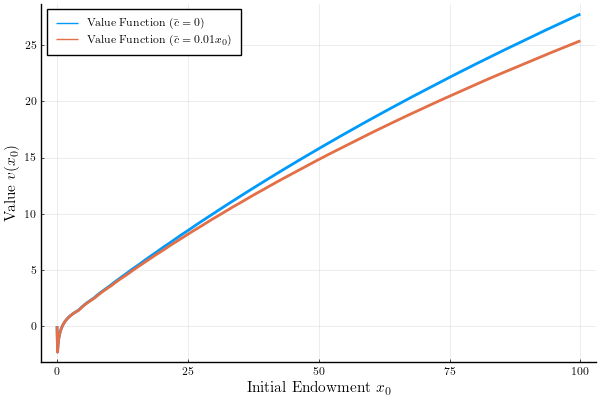
\includegraphics{macro_hw3_code/value_function_subsistence.png} \caption{Value to the Farmer when $\bar{c} = 0.01 x_0$} \label{fig:value_subs}\end{figure}
\end{enumerate}


\paragraph{Code.} The Julia code I used to complete this problem is below. It runs entirely in approximately 0.98 seconds.


\lstinputlisting[language=Julia]{macro_hw3_code/main.jl}











































\end{document}